% vim:ft=tex:
%
\documentclass[12pt]{article}
\usepackage{amsmath,amsfonts,amsthm}
\usepackage{graphicx}
\usepackage[top=2cm,left=1.5cm,right=1.5cm,bottom=2cm]{geometry}
\usepackage{longtable}

\title{
	JuliaSmoothOptimizers \\ SolverBenchmark.jl
}
\author{
	Abel Soares Siqueira \\ Dominique Orban
}
\date{ }

\begin{document}
\maketitle

\section*{Output of solver alpha}

\documentclass[varwidth=20cm,crop=true]{standalone}
\usepackage{longtable}
\begin{document}
\begin{longtable}{rrrrrrr}
\hline
id & name & status & f & t & iter & irrelevant \\\hline
\endhead
\hline
\multicolumn{7}{r}{{\bfseries Continued on next page}}\\
\hline
\endfoot
\endlastfoot
\(     1\) & prob001 & failure & \(-6.89\)e\(-01\) & \( 6.24\)e\(+01\) & \(    20\) & \(-7.51\)e\(-01\) \\
\(     2\) & prob002 & failure & \(-7.63\)e\(-01\) & \( 3.53\)e\(+02\) & \(    80\) & \( 1.20\)e\(+00\) \\
\(     3\) & prob003 & first\_order & \( 3.97\)e\(-01\) & \( 7.68\)e\(+02\) & \(    10\) & \( 1.48\)e\(+00\) \\
\(     4\) & prob004 & first\_order & \( 8.12\)e\(-01\) & \( 4.31\)e\(+01\) & \(    60\) & \( 4.56\)e\(-01\) \\
\(     5\) & prob005 & first\_order & \(-3.46\)e\(-01\) & \( 2.68\)e\(+02\) & \(    60\) & \(-1.30\)e\(-01\) \\
\(     6\) & prob006 & first\_order & \(-1.88\)e\(-01\) & \( 6.68\)e\(+01\) & \(    60\) & \( 7.00\)e\(-01\) \\
\(     7\) & prob007 & first\_order & \(-1.61\)e\(+00\) & \( 1.57\)e\(+02\) & \(    50\) & \(-8.73\)e\(-01\) \\
\(     8\) & prob008 & first\_order & \(-2.48\)e\(+00\) & \( 6.05\)e\(+02\) & \(    10\) & \(-4.10\)e\(-01\) \\
\(     9\) & prob009 & first\_order & \( 2.28\)e\(+00\) & \( 1.36\)e\(+02\) & \(    10\) & \(-6.92\)e\(-01\) \\
\(    10\) & prob010 & failure & \( 2.20\)e\(-01\) & \( 8.38\)e\(+02\) & \(    80\) & \( 1.52\)e\(-01\) \\\hline
\end{longtable}
\end{document}


\section*{Joined output}

\begin{longtable}{rrrrrrrrrrr}
\hline
id & name & flag\_alpha & f\_alpha & t\_alpha & flag\_beta & f\_beta & t\_beta & flag\_gamma & f\_gamma & t\_gamma \\\hline
\endhead
\hline
\multicolumn{11}{r}{{\bfseries Continued on next page}}\\
\hline
\endfoot
\endlastfoot
\(     1\) & prob001 & failure & \(-6.89\)e\(-01\) & \( 6.24\)e\(+01\) & first\_order & \(-4.83\)e\(-01\) & \( 3.92\)e\(+02\) & failure & \(-9.99\)e\(-01\) & \( 6.97\)e\(+02\) \\
\(     2\) & prob002 & failure & \(-7.63\)e\(-01\) & \( 3.53\)e\(+02\) & first\_order & \(-1.16\)e\(+00\) & \( 4.79\)e\(+02\) & first\_order & \( 1.03\)e\(+00\) & \( 4.35\)e\(+02\) \\
\(     3\) & prob003 & first\_order & \( 3.97\)e\(-01\) & \( 7.68\)e\(+02\) & first\_order & \(-2.14\)e\(-01\) & \( 6.82\)e\(+01\) & first\_order & \(-1.16\)e\(+00\) & \( 9.86\)e\(+02\) \\
\(     4\) & prob004 & first\_order & \( 8.12\)e\(-01\) & \( 4.31\)e\(+01\) & first\_order & \(-1.37\)e\(+00\) & \( 4.80\)e\(+02\) & first\_order & \( 5.34\)e\(-01\) & \( 9.97\)e\(+02\) \\
\(     5\) & prob005 & first\_order & \(-3.46\)e\(-01\) & \( 2.68\)e\(+02\) & first\_order & \(-1.54\)e\(+00\) & \( 4.68\)e\(+02\) & first\_order & \(-3.08\)e\(-01\) & \( 5.08\)e\(+02\) \\
\(     6\) & prob006 & first\_order & \(-1.88\)e\(-01\) & \( 6.68\)e\(+01\) & first\_order & \(-1.23\)e\(+00\) & \( 4.52\)e\(+02\) & first\_order & \( 9.86\)e\(-01\) & \( 2.16\)e\(+02\) \\
\(     7\) & prob007 & first\_order & \(-1.61\)e\(+00\) & \( 1.57\)e\(+02\) & first\_order & \(-1.96\)e\(+00\) & \( 6.44\)e\(+02\) & first\_order & \(-1.19\)e\(+00\) & \( 8.59\)e\(+02\) \\
\(     8\) & prob008 & first\_order & \(-2.48\)e\(+00\) & \( 6.05\)e\(+02\) & failure & \(-4.73\)e\(-01\) & \( 6.69\)e\(+02\) & first\_order & \( 6.80\)e\(-01\) & \( 9.05\)e\(+02\) \\
\(     9\) & prob009 & first\_order & \( 2.28\)e\(+00\) & \( 1.36\)e\(+02\) & first\_order & \( 1.34\)e\(+00\) & \( 9.48\)e\(+01\) & failure & \( 2.04\)e\(-03\) & \( 4.35\)e\(+02\) \\
\(    10\) & prob010 & failure & \( 2.20\)e\(-01\) & \( 8.38\)e\(+02\) & first\_order & \( 8.08\)e\(-01\) & \( 9.49\)e\(+02\) & first\_order & \(-4.78\)e\(-01\) & \( 6.59\)e\(+01\) \\\hline
\end{longtable}


\section*{Profiles}

\begin{center}
  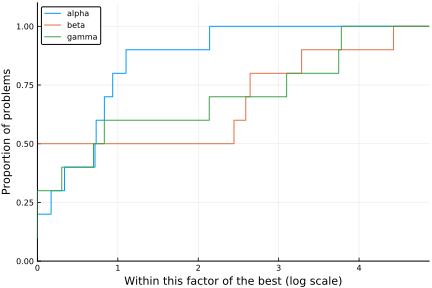
\includegraphics[width=0.66\textwidth]{profile1}

  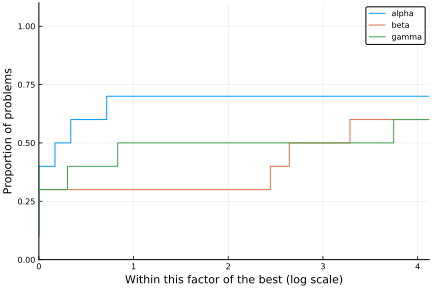
\includegraphics[width=0.66\textwidth]{profile2}
\end{center}

\end{document}
